\begin{frame}
    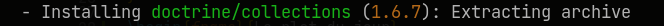
\includegraphics[width=\textwidth]{screenshots/Screenshot_20210520_104535.png}
    \pause
    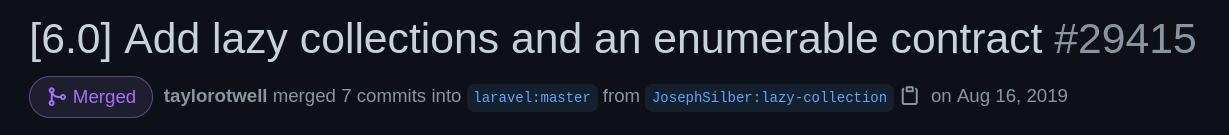
\includegraphics[width=\textwidth]{screenshots/Screenshot_20210520_101402.png}
    
\includegraphics[width=\textwidth]{screenshots/Screenshot_20210520_101458.png}
\end{frame}

\begin{frameC}{Pourtant, on a déjà tout en PHP!}

\end{frameC}

\begin{frame}{Pourquoi}{Oui mais...}
    Tout cela est déjà possible avec des simples boucles.

    En effet.

    Il y a plusieurs types de profils.
    - Les business
    - Les passionnes

    L'avantage du business c'est qu'il delivre vite
    L'avantage des passionnes c'est qu'il favoriseront plutot
    des aspects comme la sémantique et la lisibilite du code.

    Les désavantages ne sont pas nécessaires ici, je laisse aux
    participants le soin de tirer leurs conclusions.

    Du coup, comme je me situe dans le dernier profil, j'ai cree
    loophp/collection.
\end{frame}

\begin{frame}{Pourquoi}{Gérer des ensembles de données}
    PHP dispose de fonctions natives propices à l'itération

    \begin{itemize}[<+->]
        \item Les fonctions \texttt{array\_*} (\textit{$\pm$ 52 disponibles})
        \begin{itemize}[<+->]
            \item \texttt{array\_map()}
            \item \texttt{array\_filter()}
            \item \texttt{array\_reduce()}
            \item \texttt{array\_walk()}
        \end{itemize}
    \item \texttt{iterator\_to\_array()}
    \end{itemize}
\end{frame}

\begin{frame}{Pourquoi}{Gérer des ensembles de données}
    PHP dispose de structures natives propices à l'itération

    \begin{itemize}[<+->]
        \item Tableaux (\texttt{array})
        \item Objects/Interfaces (\texttt{ArrayObject}, \texttt{ArrayAccess})
        \item Itérateurs
        \item Générateurs
    \end{itemize}
\end{frame}

\begin{frame}{Pourquoi}{Gérer des ensembles de données}
    PHP dispose de structures natives propices à l'itération

    \begin{itemize}[<+->]
        \item \texttt{for}
        \item \texttt{foreach}
        \item \texttt{while}
        \item \texttt{do-while}
    \end{itemize}
\end{frame}

\begin{frameC}{Oui, mais\ldots}

\end{frameC}

\begin{frame}{Pourquoi}{Des incohérences?}
    \begin{itemize}[<+->]
        \item \texttt{array\_map()}
        \item \texttt{array\_filter()}
        \item \texttt{array\_reduce()}
        \item \texttt{array\_walk()}
    \end{itemize}
\end{frame}

\begin{frame}{Pourquoi}{Des incohérences?}
    \begin{itemize}[<+->]
        \item Uniquement pour les \texttt{array}
        \item Inconsistance des fonctions (\texttt{array\_*()})
        \item Ordre des arguments (\textit{Sera probablement different avec PHP 8})
        \begin{itemize}[<+->]
            \item \texttt{array\_map(\$callable, \$array)}
            \item \texttt{array\_map(\$array, \$callable)}
        \end{itemize}
        \item Inconsistance des callbacks
        \item Pas de vérification des types
        \item Performances
        \item Pas de gestion des erreurs
    \end{itemize}
\end{frame}

\begin{frame}{Incohérences}{\texttt{array\_map()}}
    Un array est composé de\ldots

    \begin{itemize}[<+->]
        \item clés (\texttt{\$key})
        \item valeurs (\texttt{\$value})
    \end{itemize}

    \pause[\thebeamerpauses]

    Cependant\ldots

    \pause[\thebeamerpauses]

    \begin{itemize}[<+->]
        \item Signature: \texttt{array\_map(\$callable, \$array)}
        \item Signature de \texttt{\$callable}: \texttt{\$callable(\$value)}
    \end{itemize}
\end{frame}

\begin{frame}{Incohérences}{Pourquoi?}
    \begin{itemize}[<+->]
        \item Un \texttt{array} est un ensemble de couple: $\left(\texttt{clé} \Rightarrow \texttt{valeur}\right)$
        \item \texttt{\$key} n'est pas passé au callback ?
    \end{itemize}
\end{frame}

\begin{frameC}{Bref\ldots}

\end{frameC}

\begin{frame}{Pourquoi}{In a nutshell}
    \begin{itemize}[<+->]
        \item On sait que PHP n'est pas parfait \pause[\thebeamerpauses] (\textit{mais qu'il va bientot l'etre :D})\pause[\thebeamerpauses]
        \item On a l'habitude et donc, on ne fait plus attention
        \item Cela ne nous empêche pas de construire de belles choses malgré tout
    \end{itemize}
\end{frame}
